%%
%% This is file `example-1.tex',
%% generated with the docstrip utility.
%%
%% The original source files were:
%%
%% drexel-thesis.dtx  (with options: `example-part')
%% 
%% This is a generated file.
%% 
%% Copyright (C) 2010 W. Trevor King
%% 
%% This file may be distributed and/or modified under the conditions of
%% the LaTeX Project Public License, either version 1.3 of this license
%% or (at your option) any later version.  The latest version of this
%% license is in:
%% 
%%    http://www.latex-project.org/lppl.txt
%% 
%% and version 1.3 or later is part of all distributions of LaTeX version
%% 2003/06/01 or later.
%% 

\chapter{Neuron population activity encoding and transport via traveling waves in neuronal systems }

Individual neurons in the brain are tuned to fire upon specific events such as visual stimuli of a particular type \citep{Hubel1962} .
However, even neurons that are tuned to a specific stimulus show variability in their firing rate and timing when the same stimulus is repeatedly applied \citep{Georgopoulos1982}\citep{Newsome1989}.
This indicates that information in the brain is represented by the firing dynamics of populations of many neurons.
This population coding may take the form of variations in the average firing rate of the neurons in the population (rate coding) or variations in the synchronization between spikes (temporal coding).
The temporal and rate coding may also have a functional relation, i.e. through Hebbian learning \citep{Basawaraj2019}.
Various methods of decoding the information in these population dynamics have been studied \citep{Deneve1999}\citep{Xu2019}, and population dynamics are incorporated into modern theories of neural computation \citep{Pitkow2017}\citep{Nadeau2020}.

Traveling waves of neuronal activation have been observed in the cortex as reviewed in \citet{Muller2018}.
Various functional roles have been proposed for these traveling waves including spatiotemporal processing in the visual cortex \citep{wu2008}\citep{Muller2014}, place field coordination in the hippocampus \citep{lubernov2009}, and memory consolidation during sleep \citep{Dickey2021}.
Traveling waves have been shown to carry information in the  motor cortex \citep{Rubino2006} and visual cortex \citep{Besserve2015}.
These waves can provide synchronous activations of a population to serve functions such as gating perception of low-contrast images \citep{Davis2020}.
In addition to extensive observations in vivo, traveling waves have also been observed in neuronal network simulations at the mesoscopic level in simple one-dimensional systems \citep{Wilson1973}\citep{Golomb1999} and two-dimensional sheets \citep{keane2015}.
Traveling waves have also been studied in large-scale simulations of the entire brain \citep{Roberts2019}.

Previous studies have used one-dimensional structures largely for their computational or analytic simplicity. 
Consideration of a quasi one-dimensional system may seem as an unnecessary complication, but there is no a priori reason that quasi one-dimensional traveling waves may not be found in vivo.
Of interest, there are regions of the brain where there are what seem to be quasi one-dimensional structures \citep{mountcastle1997}\citep{Cruz2009} typically called micro- or minicolumns. 
These minicolumns are aligned perpendicular to the pia and can be hundreds of microns long.  
Although their relevance to cognition and function is still being debated \citep{horton2005}\citep{buxhoeveden2002}, it is possible that they can sustain traveling waves.

Here we consider how quasi one-dimensional neuronal structures could encode and transmit population activity via traveling waves.
We perform computational experiments using a quasi one-dimensional model we call a Small Columnar Ensemble (SCE), first reported in , with a network of Izhikevich neurons \citep{izhikevich2003} using the same local connectivity model as \citep{maass2002}.
We have previously shown that this model supports stimulus-evoked traveling waves across a variety of model parameters.
We now demonstrate that input from a population of neurons, simulated as Poisson spike trains, can evoke traveling waves in our quasi one-dimensional system.
The number of waves per second that span the SCE, which we term the wave arrival rate, increases as the average firing rate of the input pool of neurons is increased.
The plot of wave arrival rate versus input population firing rate resembles the activation functions of either a single neuron or a population of neurons.
This leads us to consider the SCE to have a nonlinear activation function in terms of input population rate, and to consider the SCE as encoding the input population firing rate into the wave arrival rate.

Just as a single neuron may be susceptible to noise or damage, a single SCE may also be an unreliable means of encoding and transmitting population rate information.
We therefore look at morphologies of multiple redundant SCE to enable reliable encoding and transport.
We find that simply increasing the cross-section of the SCE ...

We performed a series of computational experiments to determine how our SCE can encode and transmit population activity.
We first verified that our population of Poisson neurons can invoke traveling waves in a single SCE.
The wave rate in the single SCE was found to be proportional to the instantaneous firing rate of the population of Poisson neurons.
The relationship between population activity and wave rate resembled the activation functions of both single neurons and populations of neurons, so we termed this relationship the activation function of the SCE.
The activation function of the SCE showed significant variation across trials with randomly generated stimuli, indicating that the population rate encoding was not reliable.
We then created SCE with larger cross-section (X and Y extents) with varying topologies and observed that an ensemble of multiple SCE with loose coupling between them reduces the variation in the activation function.

\subsection{Traveling waves are evoked by population activity}
Our first configuration is an SCE with dimensions $2x2x40$ (X/Y/Z).
The SCE parameters are $C=0.5$, $\lambda=2.5$, $\kappa=0.1$, $K^{SCE}=24$ and $K^{stim}=6$.
The other parameters are fixed for all experiments as described in Methods.

We stimulated the SCE using several instantaneous firing rates for the input population.
Traveling waves are evoked in the SCE for higher firing rates (Figure \ref{fig:sce_raster}).

\begin{figure}[!htb]
 \centering
 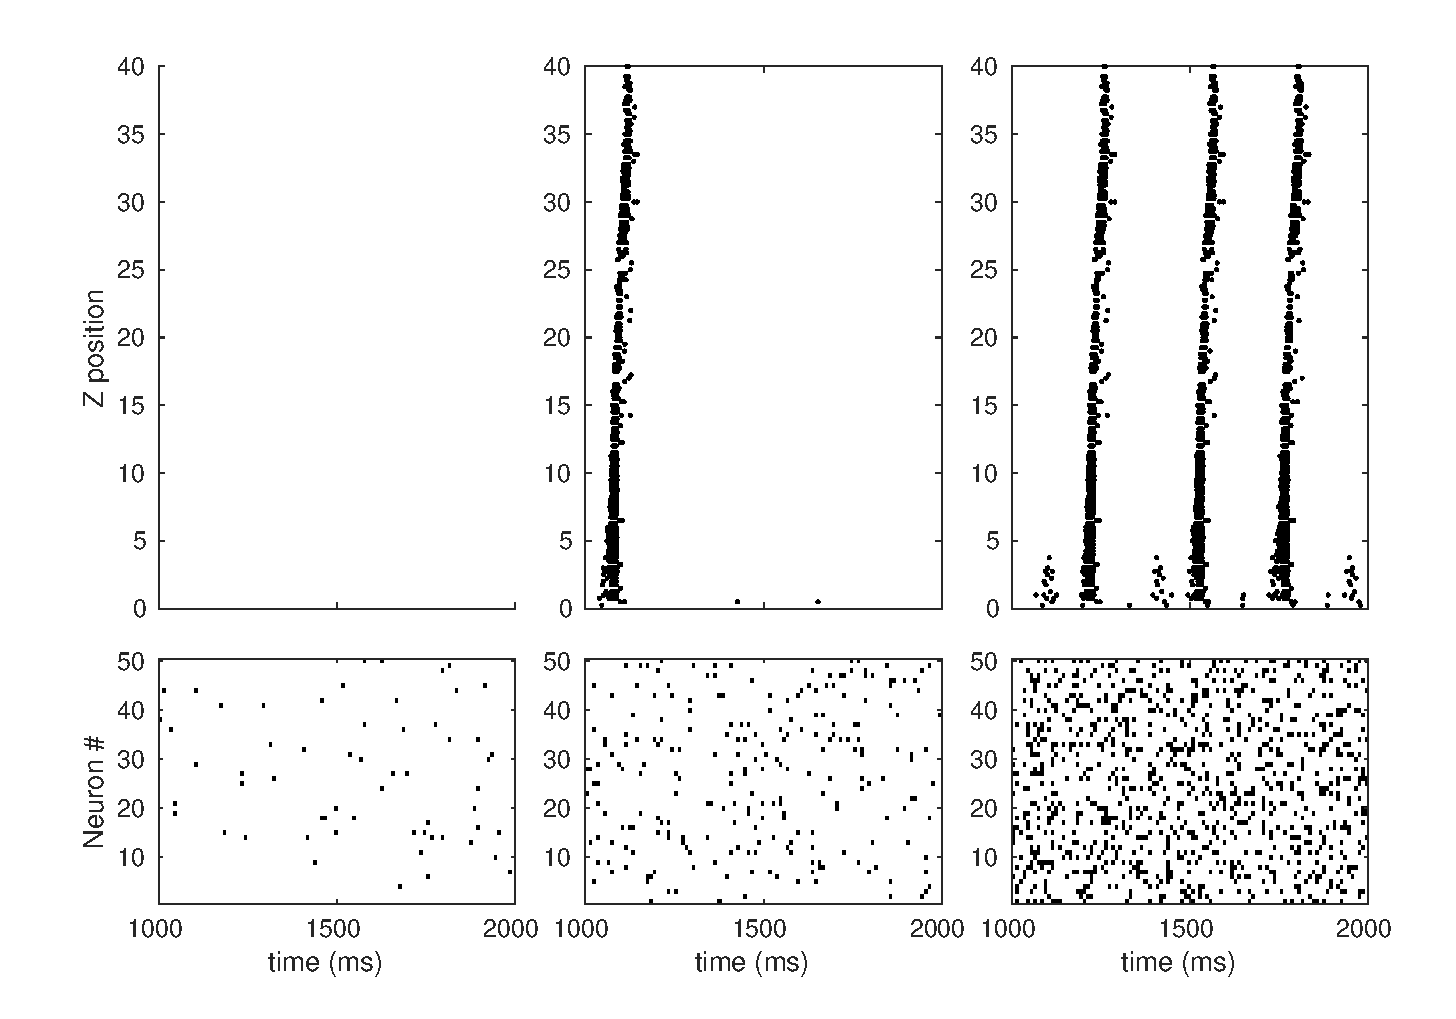
\includegraphics[width=\textwidth]{fig/SCE_2x2_FRE_rasters}
 \caption{Poisson spike trains in the input population (bottom) evoke traveling waves in the SCE (top). Raster plots are shown for firing rates of 1 spike/second (left), 5 spikes/second (middle) and 21 spikes/second (right).  }
 \label{fig:sce_raster}
\end{figure}

\FloatBarrier

\subsection{The SCE possesses an activation function}
We stimulated the SCE with instantaneous firing rates from 1 to 21 spikes/second, with 100 random inputs created for each firing rate.
The resulting waves rates are shown in Figure \ref{fig:sce_activation_function}.
The mean wave rate showed a clear trend that is similar to a logarithmic curve. 
It also resembled the population activation rate shown in \citet{Trappenberg2010} Eq. 3.43 for the population response to slowly varying inputs:
\begin{align}
 g(x) &= \frac{1}{t^{ref}-\tau \log{(1-\frac{1}{\tau x})}}
\end{align}
where $t^{ref}$ is an absolute refractory period and $\tau$ is the charateristic response time.
We therefore consider our SCE to have an nonlinear activation function when stimulated by a  population of neurons.
This demonstrated that the SCE can be said to encode the population rate into the wave rate in a analogous manner to which single neurons and populations of neurons encode their stimulus strength into their firing rate.

\begin{figure}[!htb]
 \centering
 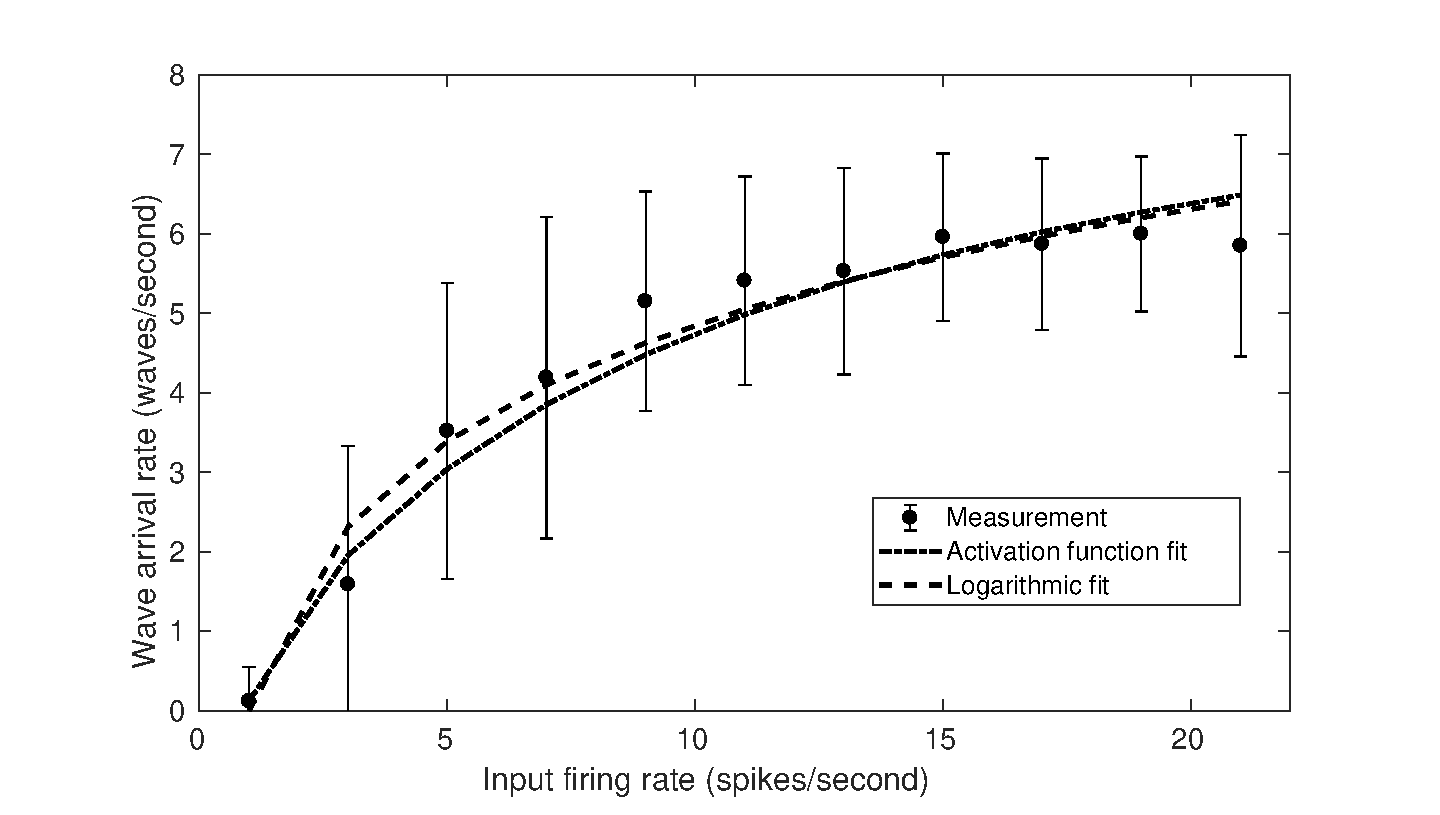
\includegraphics[width=\textwidth]{fig/SCE_2x2_FRE}
 \caption{The SCE encodes the input population firing rate into the wave arrival rate. }
 \label{fig:sce_activation_function}
\end{figure}

Although the mean wave rates showed a clear trend, the trial-to-trial wave rates were highly variable. 
This indicates that our SCE would not reliably encode population rate into wave rate.

\FloatBarrier

\subsection{Adding redundant columns to the SCE can reduce variability in the activation function}
Like our SCE, individual neurons also have variable firing responses to identical stimuli.
This variability is one of the key motivations for the population activity theories of information encoding in the cortex.
We next followed a similar approach and investigated the activation function of a population of multiple redundant SCE.
Several populations of SCE were generated with different distance (and therefore connectivity), between the individual SCE.
We found that a population of four SCE, with the individual SCE separated by $2\lambda$, produced a much smoother activation function.
A population of four widely separated SCE with no connectivity between them was still highly variable.


\begin{figure}[!htb]
 \centering
 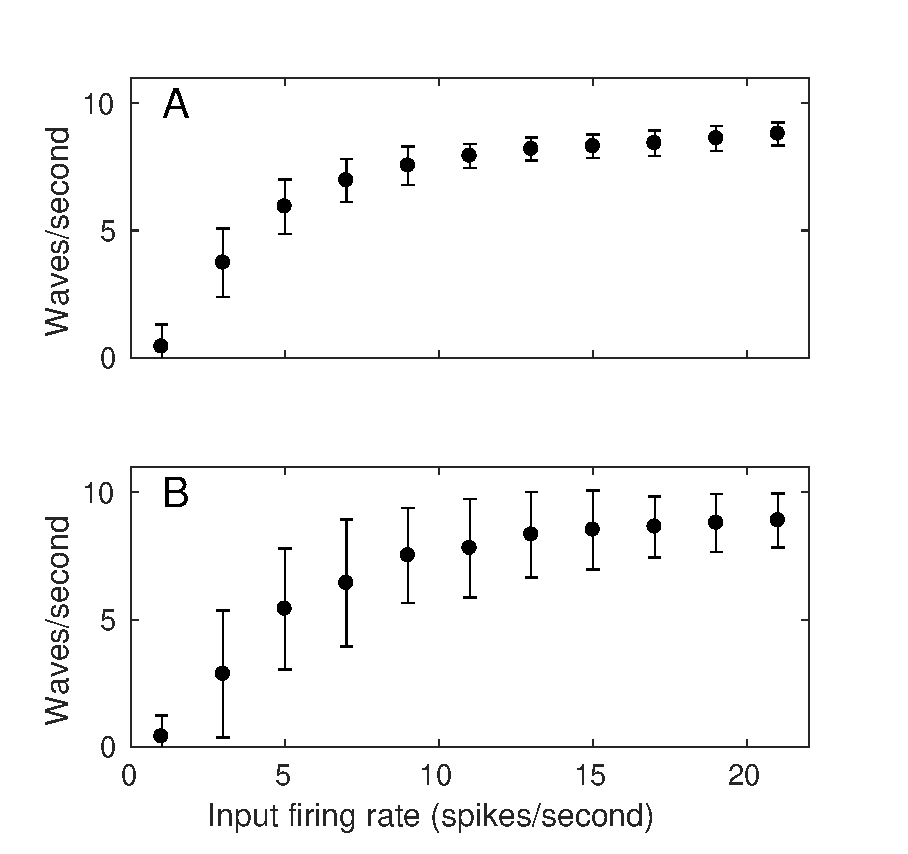
\includegraphics[width=\textwidth]{fig/OneLambdaFourLambda}
 \caption{Activation functions of a population of 4 SCEs. 
	    A: When the SCE are spaced $2\lambda$ apart the activation function shows greatly reduced variability. 
	    B: When the SCE are widely spaced with no connectivity between the SCE there is still substantial variability in the activation function.}
 \label{fig:sce_4x4_coupled_activation_function}
\end{figure}

\FloatBarrier


\endinput
%%
%% End of file `example-1.tex'.
